The metal films were deposited directly on substrates by means of a plasma
sputtering process.  It is through this process that the surface roughness
of the metal film was also controlled.  Our base process consists of
top-down sputtering in Argon plasma at a pressure of \SI{1}{\milli\torr}
and a flow rate of \SI{12}{STP}.  The deposition rates were
\SI{6.60}{\angstrom\per\second} for gold and
\SI{5.88}{\angstrom\per\second} for silver at 150 and \SI{66}{\watt} DC,
respectively.  During sputtering, the samples were rotated at \SI{50}{RPM}.
Adhesion of the metal films to both glass and flouropolymer substrates was
found to be very poor, but we did not attempt to address this issue.
Instances of film-substrate separation were rare enough (4-5 times amongst
hundreds of experiments) that it did not warrant the effort given our
careful attention to stresses on the film.  Typical surface qualities are
shown in \Figure{fig:semsputter} for both gold and silver.  
\begin{figure}
\centering
\includegraphics[keepaspectratio,width=5cm]{experimental/figures/SEM-nanoparticles.pdf}
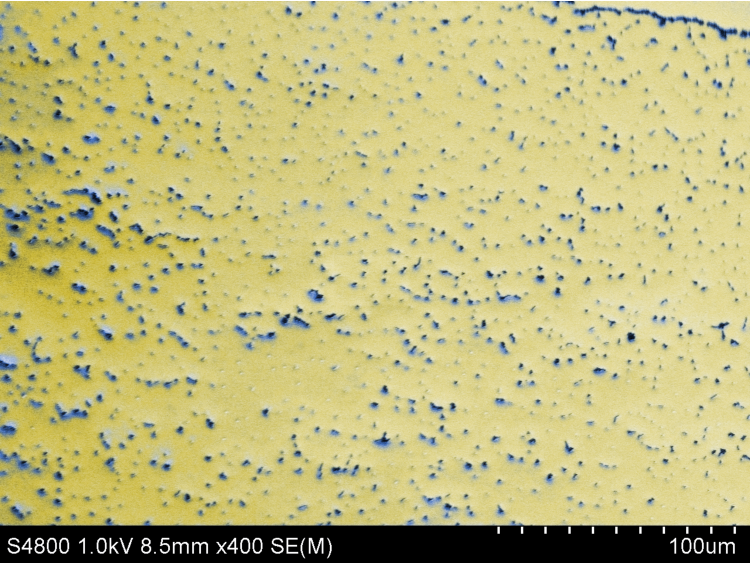
\includegraphics[keepaspectratio,width=5cm]{experimental/figures/SEM-holesa.pdf}
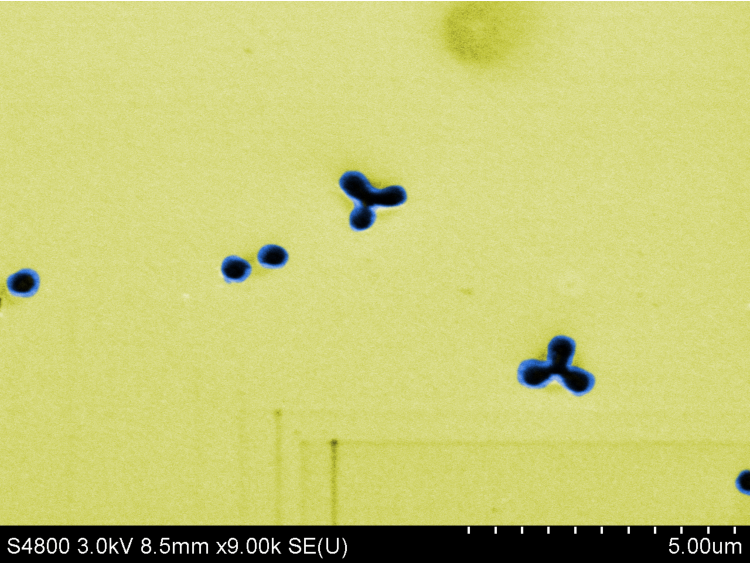
\includegraphics[keepaspectratio,width=5cm]{experimental/figures/SEM-holesb.pdf}
\caption{SEM images of typical films produced with the plasma sputtering
technique using the base set of parameters described in the text.}
\label{fig:semsputter}
\end{figure}

The substrate material consisted of \SI{12}{\milli\meter} diameter BK7
glass slides with nominal suface roughness of XXX.  They were cleaned in
the following way.  A \SI{2}{\percent} solution of Hellmanex II was first
prepared in a pyrex beaker with a volume of \SI{25}{\milli\liter} and
heated to a temperature of \SI{60}{\celsius} on a hot plate.  The BK7
slides are placed in this solution on the hot plate and washed for
\SI{300}{\second}, swirling gently by hand occasionally.  The container
with the solution and slides was then sonicated for \SI{300}{\second}.
After sonication, the slides are removed from the solution and washed
liberally with distilled water and dried under a nitrogen stream.  Cleaned
glass slides were stored individually on top of a small
\SI{1}{\milli\meter\cubed} piece of PDMS plasma bonded to a microscope
slide, and batches kept in a dark box until use.  Slides sputtered with
metal films were stored in the same manner, but always used within one week
of preparation.

Once deposited, while a gold film will last virtually forever if left
undisturbed, the silver film should slowly lose its integrity due to
oxidation.  This has not been observed, as new films are easily created at
regular intervals.  

Since the metal films are very thin and SPR is particularly sensitive to
surface conditions, care must be taken not to damage the films.  Once
prepared, they cannot be touched in any way.  Cleaning them with lens
tissue, even using the drag and drop method, destroys their integrity.  Dry
nitrogen seems to be the only option for removing dust if contaminated, but
prevention is always preferable.

\subsection{Prisms}
To prepare prisms for sputtering, any existing film must first be
removed.  Silver films are removed by subjecting them to a solution of
\SI{70}{\percent} \ce{HNO3}.  For this is was determined unnecessary to
submerse the entire prism.  Rather, the prism is positioned in a small
Pyrex dish hypotenuse side up and the \ce{HNO3} solution pipetted on.
Surface tension will prevent a small amount of solution from flowing off
the surface; in this way it may be covered in its entirety.  After
approximately \SI{60}{\second} the silver has been eaten away and the
solution is removed.  The same procedure was carried out for the removal of
gold films, but in this case the dissolving solution was freshly prepared
aqua regia, composed of a 1:3 ratio of \ce{HNO3} to \ce{HCl}.

After any old films have been removed, the prisms are sonicated in acetone
to remove any organic contaminants and rinsed in ultra-pure dry acetone.
The surface is then cleaned with methanol and lens tissue using the drag
and drop method.
